\section{Conceptos generales}
\subsection{Fluidos}
\subsubsection{Definición de un fluido}
Un fluido es una sustancia que siempre se deforma continuamente cuando se somete a un esfuerzo cortante, sin importar qué tan pequeño sea dicho esfuerzo.\\

Tiene \textbf{propiedades} que lo caracterizan y definen el estado en el que se encuentra, pudiendo determinar su comportamiento. Algunas de estas propiedades son: \\
\begin{center}
	\begin{tabular} {r l}
		Densidad & $\rho = \dfrac{m}{V}$\\
		Viscosidad & $\mu$\\
		Peso & $P$\\
		Peso específico & $\gamma$ \\
		Temperatura & T \\
	\end{tabular}
\end{center}


\subsubsection{Ecuación de Newton para los fluidos}
Para obtener la ecuación de newton para los fluidos, se plantea un sistema en el que un fluido se entra entre dos placas paralelas separadas por una cierta distancia. La placa inferior es fija y a la superior se le aplica una fuerza $F$ lo que produce un esfuerzo cortante en el fluido, y a su vez establece una velocidad en la placa superior.

Si la fuerza $F$, por más pequeña que sea, hace que la placa se mueva permanentemente, entonces la sustancia es un fluido.

\begin{figure}[h]
	\centering
	\begin{subfigure}[b]{0.45\linewidth}
		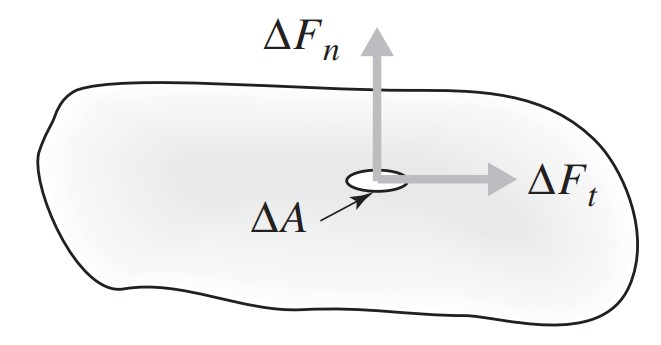
\includegraphics[width= .7\linewidth]{cortante2}
	\end{subfigure}
	\begin{subfigure}[b]{0.45\linewidth}
		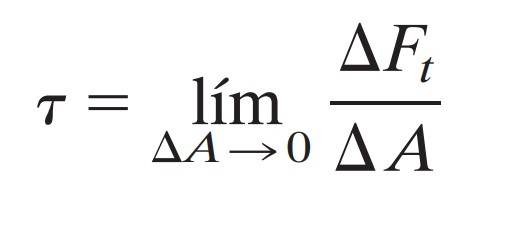
\includegraphics[width= .5\linewidth]{cortante1}
	\end{subfigure}
	\caption{Esfuerzo cortante}
\end{figure}

Manteniendo ciertas cantidades constantes, como la viscosidad del fluido, el area de las placas, la distancia entre ellas y la velocidad de la placa superior, se llega a una expresión que relaciona la fuerza aplicada con los parámetros mencionados:
\begin{center}
	$F = \mu \dfrac{A \cdot U}{y}$
\end{center}

Considerando que el esfuerzo se calcula como la fuerza aplicada en un área $\tau = \sfrac{F}{A}$:
\begin{center}
	$\tau = \mu \dfrac{U}{y}$;\\ Y en forma diferencial, $\tau = \mu \dfrac{du}{dy}$
\end{center}

El término $\dfrac{du}{dy}$ representa la tasa a la cual cada capa se mueve con respecto a la más próxima.\\ \vspace{.5cm}

A partir de esta definición, los fluidos se pueden clasificar como \textit{newtonianos} o \textit{no newtonianos}.


Los \textbf{newtonianos} son aquellos fluidos donde su viscosidad es constante, es decir, la relación entre el esfuerzo cortante ($\tau$) y la tasa de velocidad de las capas $\left(\dfrac{du}{dy}\right)$ es lineal.

Un fluido ideal se considera cuando su viscosidad es nula, por lo tanto el esfuerzo cortante requerido será nulo sin importar su movimiento.

\begin{center}
	\textbf{imagen 02}
\end{center}

\subsubsection{Viscosidad absoluta o dinámica $\mu$}
La viscosidad es una propiedad propia del fluido e indica el grado de resistencia a los esfuerzos cortantes.

En los gases, la viscosidad absoluta incrementa con la temperatura, en cambio, en los líquidos disminuye junto con esta. Esto se debe a la cohesión entre las moléculas de la sustancia (se puede completar más).

\subsubsection{Viscosidad cinemática $v$}

Es la relación entre la viscosidad absoluta y la densidad de la sustancia
\begin{center}
	$v = \dfrac{\mu}{\rho}$
\end{center}

\subsubsection{Compresibilidad}
Es la capacidad de un fluido de disminuir su volumen bajo la aplicación de una presión. Los gases son altamente compresibles mientra que los líquidos, muy poco. 

En la materia \materia se trabaja con fluidos ideales no compresibles, es decir, de viscosidad cero.

\subsubsection{Preión de vapor}
